\documentclass[a4paper, 11pt]{article}
\author{Kajetan Kaczmarek}
\usepackage{amsmath}
\usepackage{graphicx}
\usepackage{listings}
\usepackage[T1]{fontenc}
\usepackage[utf8]{inputenc}
\usepackage[polish]{babel}
\usepackage{color} %red, green, blue, yellow, cyan, magenta, black, white
\definecolor{mygreen}{RGB}{28,172,0} % color values Red, Green, Blue
\definecolor{mylilas}{RGB}{170,55,241}
\graphicspath{{Resources/}} %Setting the graphicspath
\usepackage{float}
\usepackage[caption = false]{subfig}

\lstset{language=Matlab,%
    %basicstyle=\color{red},
    breaklines=true,%
    morekeywords={matlab2tikz},
    keywordstyle=\color{blue},%
    morekeywords=[2]{1}, keywordstyle=[2]{\color{black}},
    identifierstyle=\color{black},%
    stringstyle=\color{mylilas},
    commentstyle=\color{mygreen},%
    showstringspaces=false,%without this there will be a symbol in the places where there is a space
    basicstyle = \tiny,%
    numbers=left,%
    numberstyle={\tiny \color{black}},% size of the numbers
    numbersep=9pt, % this defines how far the numbers are from the text
    emph=[1]{for,end,break},emphstyle=[1]\color{red}, %some words to emphasise
    %emph=[2]{word1,word2}, emphstyle=[2]{style},    
}



\begin{document}
\title{Sprawozdanie STP \\* Projekt nr.2 \\* 
Zadanie 9 \\*}
\maketitle
\begin{enumerate}
\item Obiekt zadany opisany jest równaniem różnicowym : \\*
\[  y(k) = b_{\tau}u(k-\tau) +  b_{\tau+1}u(k-\tau -1) -a_1y(k-1)-a_2y(k-2)  \]

\newpage
 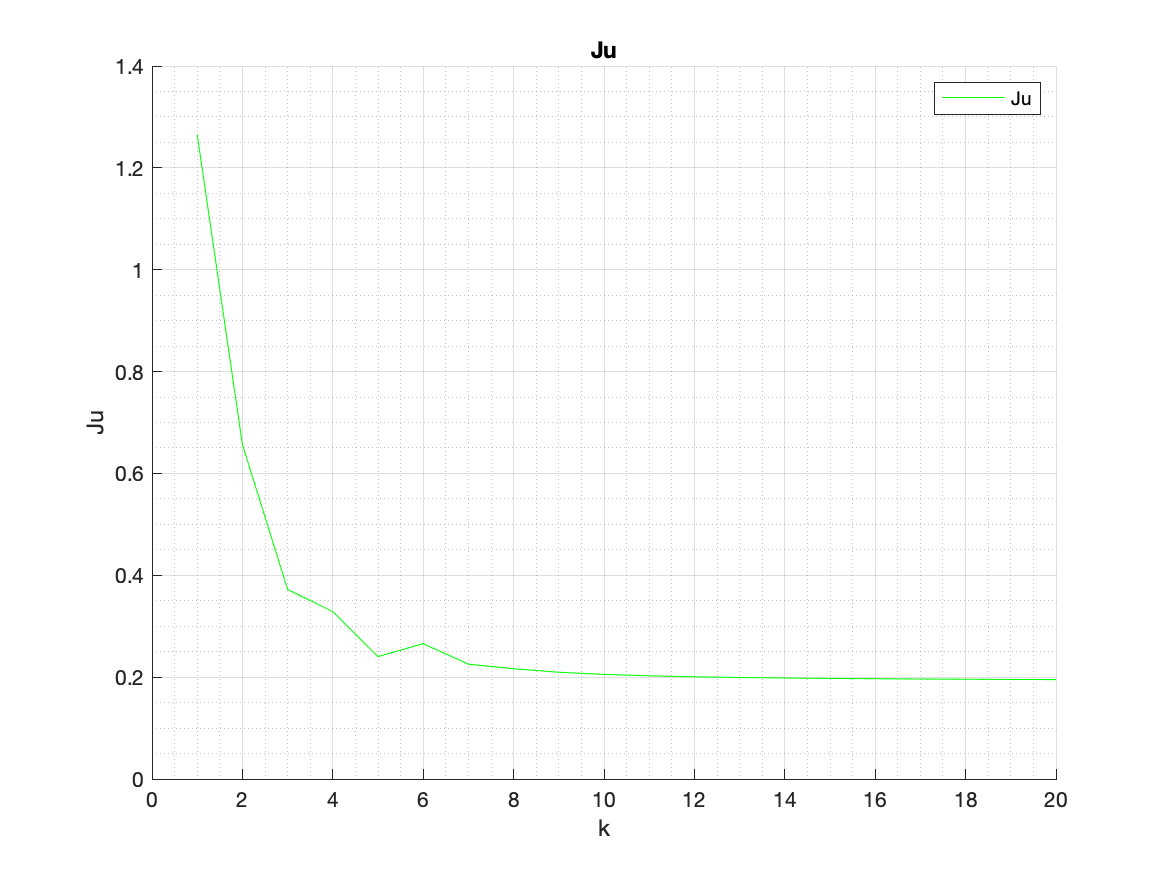
\includegraphics{./Ju.png} 
 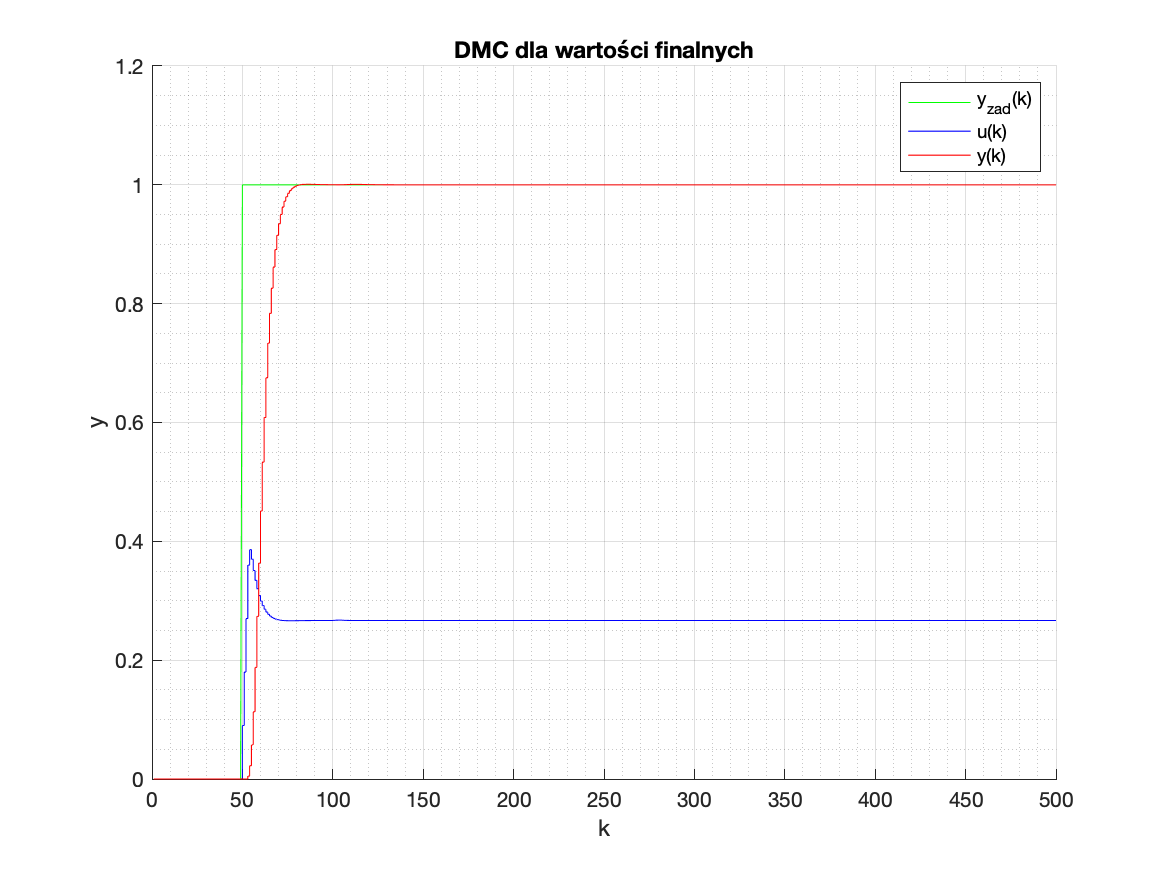
\includegraphics{./P6_3_DMC_Koncowe_.png} 
 \includegraphics{./Step.bmp} 
 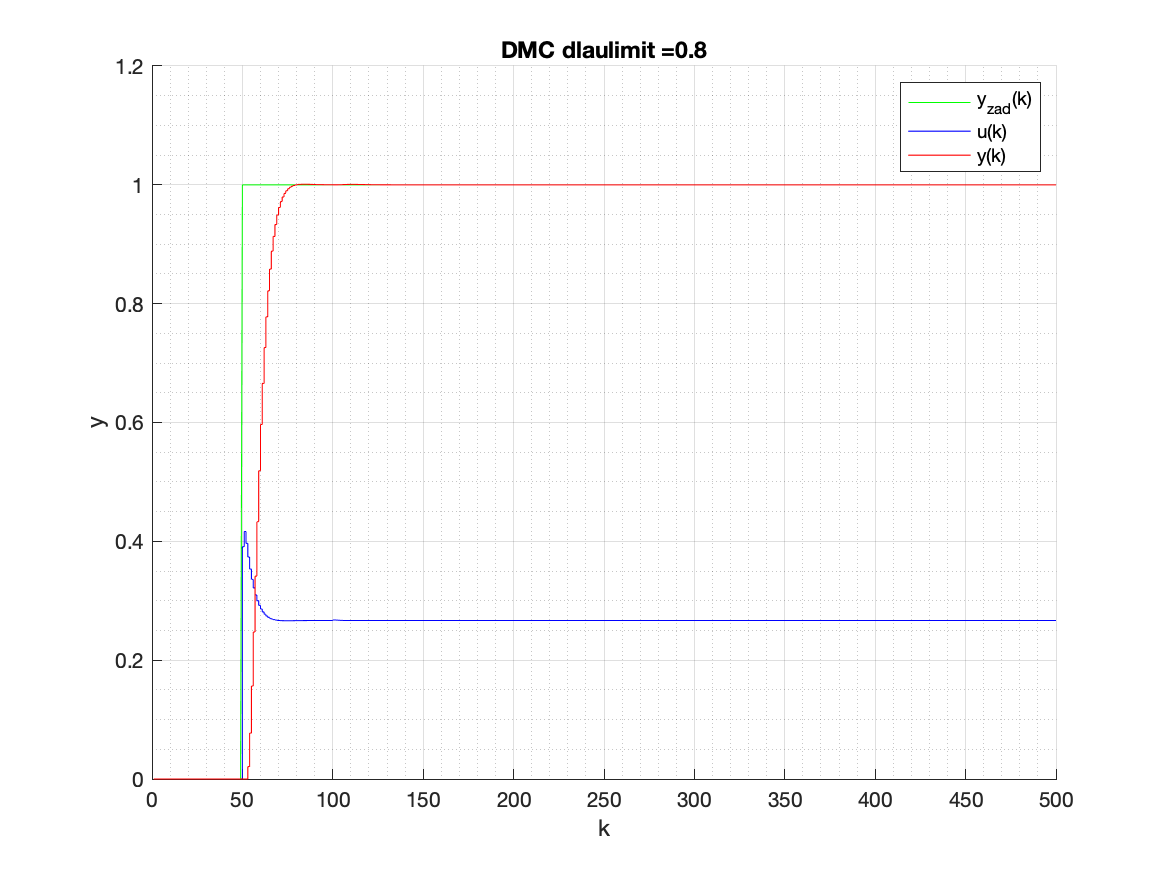
\includegraphics{./ModelsP6_ulimit/P4_DMC_ulimit_0.8.png} 
 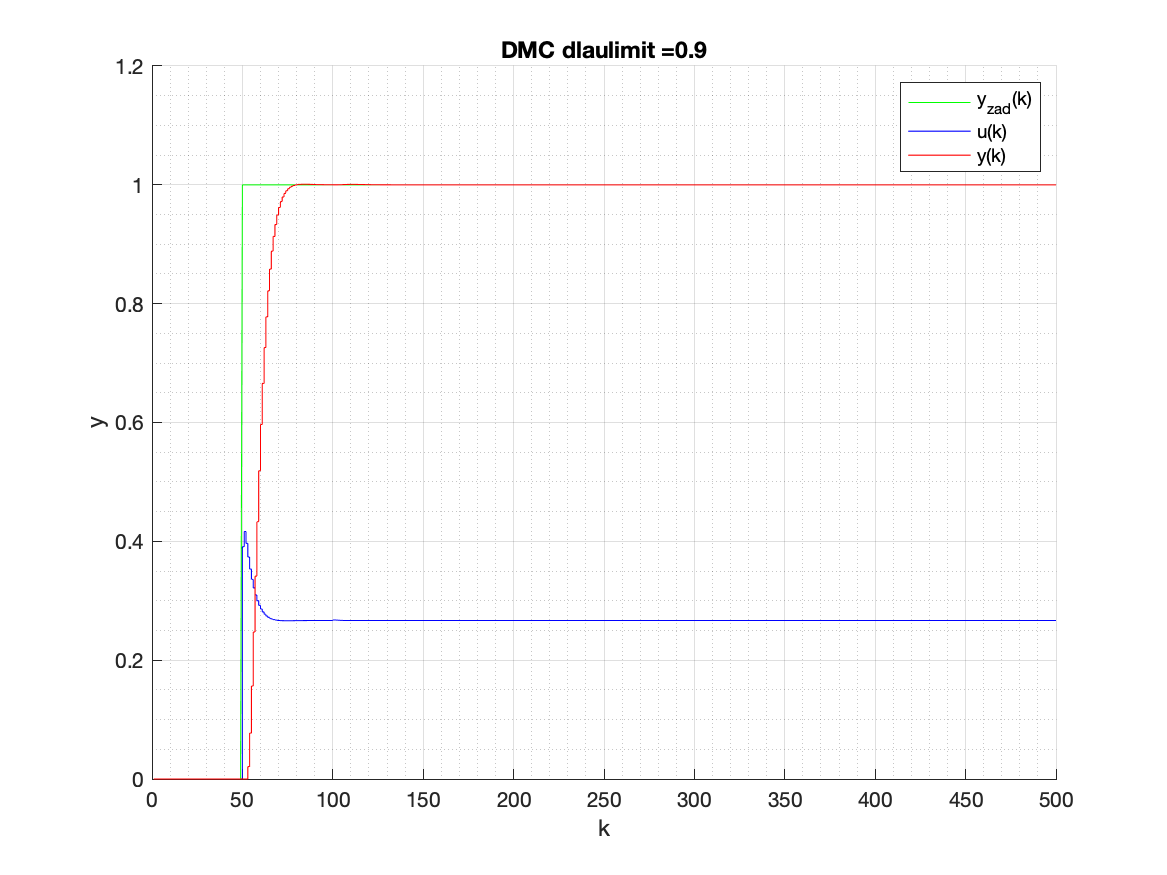
\includegraphics{./ModelsP6_ulimit/P4_DMC_ulimit_0.9.png} 
 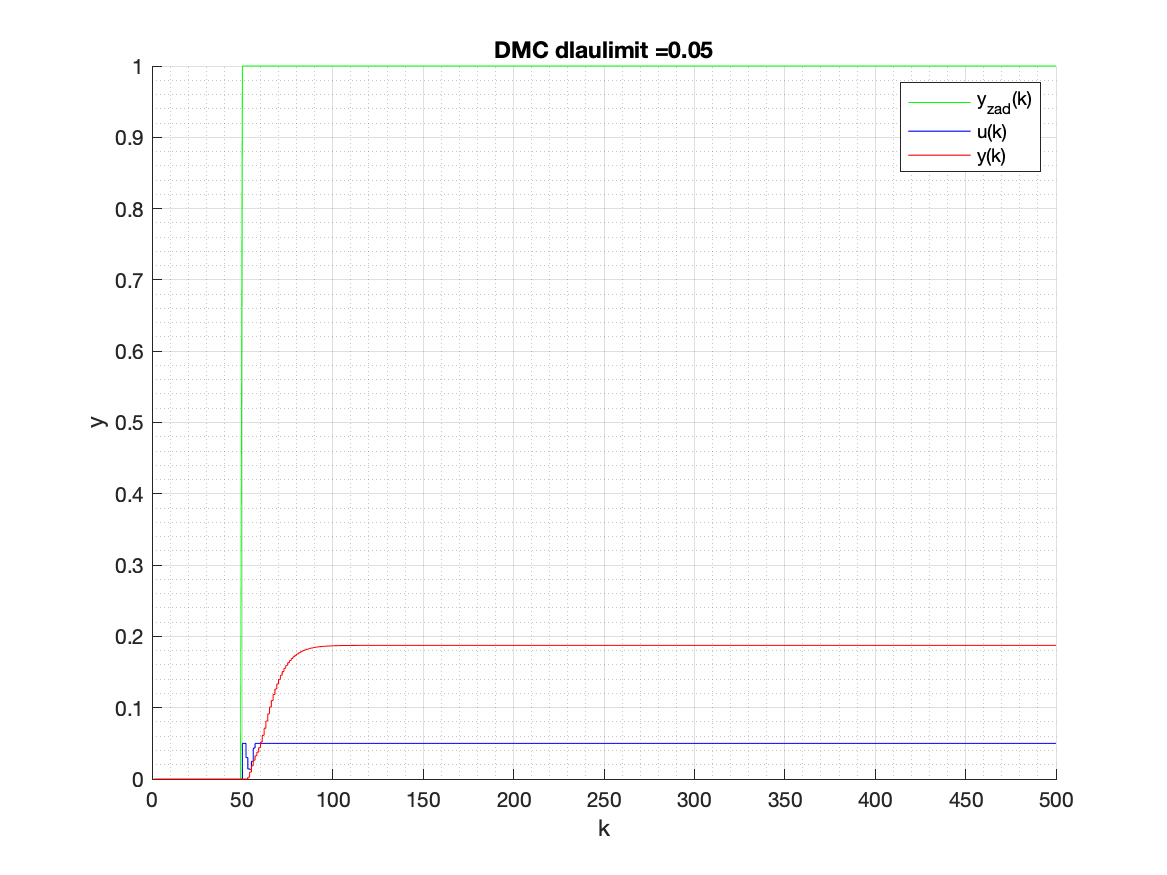
\includegraphics{./ModelsP6_ulimit/P4_DMC_ulimit_0.05.png} 
 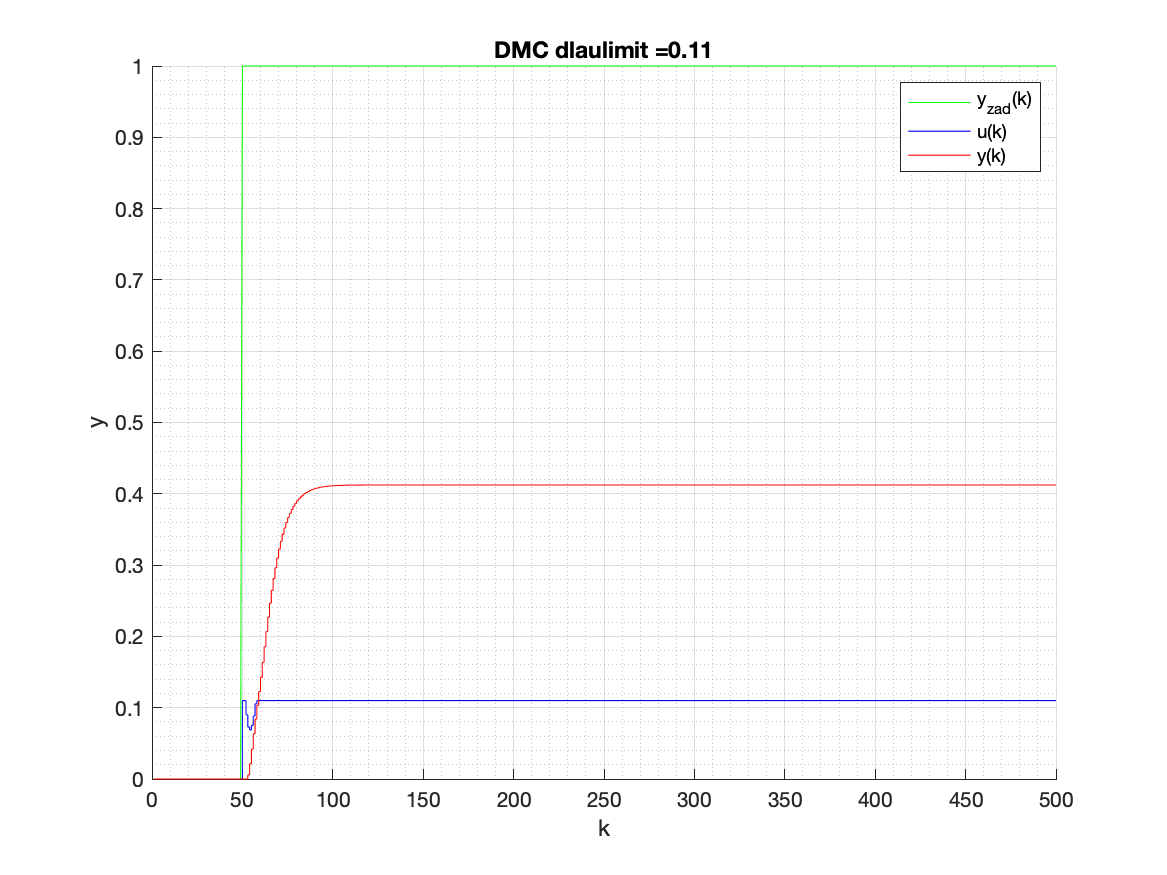
\includegraphics{./ModelsP6_ulimit/P4_DMC_ulimit_0.11.png} 
 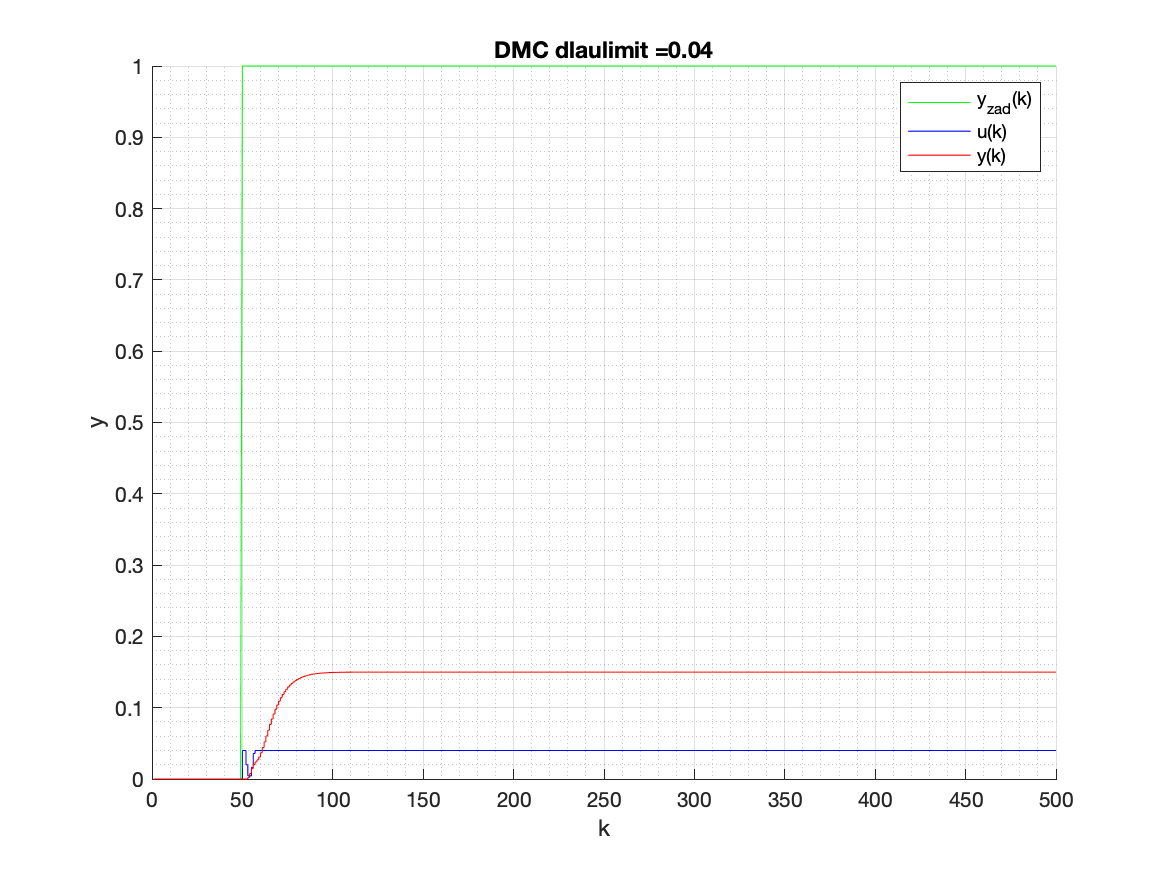
\includegraphics{./ModelsP6_ulimit/P4_DMC_ulimit_0.04.png} 

\end{enumerate}
\end{document}

